\documentclass[a4paper, 12pt]{article}

\usepackage[utf8]{inputenc}
\usepackage[german]{babel}
\usepackage{hyperref}
\usepackage[margin=3cm]{geometry}
\usepackage{graphicx}
\usepackage{graphicx}
%\usepackage{ucs}
\usepackage{minted}
\usepackage{color}
\usepackage{float}

\definecolor{mygreen}{rgb}{0,0.6,0}
\definecolor{mygray}{rgb}{0.5,0.5,0.5}
\definecolor{mymauve}{rgb}{0.58,0,0.82}

\title{2D-Zeichnen im Browser}
\author{Johannes Reuter}
\date{\today}

\pdfinfo{%
  /Title    (2D-Zeichnen im Browser)
  /Author   (Johannes Reuter)
  /Creator  (Johannes Reuter)
  /Producer (Johannes Reuter)
}

\begin{document}
\maketitle
\newpage
\tableofcontents
\newpage
\section{Motivation}
2D-Computer-Spiele haben eine lange Tradition. Von alten Gameboy-Spielen bis hin zu modernen, grafik-gewaltigen Spielen auf modernen Spielekonsolen oder iPhone-Spiele gibt es tausende verschiedene Titel, die alle nur denkbaren Spielprinzipien, Zielgruppen und Themengebiete abdecken. Seit dem Einzug des Internets in den Massenmarkt gehören dazu auch Spiele im Browser.
Diese benötigen keine Installation, sind immer auf dem neuesten Stand und daher sowohl bei Entwicklern als auch bei Kunden beliebt. Lange Zeit wurden diese Spiele fast ausnahmslos in Flash umgesetzt, was einige Probleme mit sich brachte. Zum einen muss ein Flash-Player auf dem Endgerät installiert sein; außerdem ist der Flash-Player eine proprietäre Software und daher der vollkommenen Kontrolle der Rechte-Inhaber unterworfen. Heute gibt es verschiedene offene, standardisierte Technologien, die es ermöglichen, 2D-Browserspiele ohne Einsatz kommerzieller Software zu entwickeln und anderen zur Verfügung zu stellen. Dieses Dokument gibt einen Überblick über den Stand der momentan verfügbaren Technologien und untersucht anhand Indikatoren wie Performance, Community, Browser-Unterstützung und Framework-Verfügbarkeit, welche Technologien sich heute besonders eignen, 2D-Spiele im Browser zu entwickeln.
\section{Anforderungen}
In dieser Ausarbeitung werdend die Technologien HTML5-Canvas, WebGL, DOM-Sprites und SVG untersucht. Dabei werden der Aufbau und die Arbeitsweise vorgestellt und anschließend folgende Eigenschaften bewertet.
\paragraph{Bibliotheken}
Gibt es Bibliotheken, die eine abstrakte, einfach zu verwendende API bereitstellen? Sind diese praxistauglich und umfangreich, gibt es Plugins und Erweiterungen? Nicht nur sind solche Projekte eine guter Indikator dafür, dass sich Menschen mit der Technologie beschäftigen und sie auf Tauglichkeit überprüfen, ohne solche Hilfsmittel wird es in der Praxis oft sehr schwierig, echte, große Anwendungen umzusetzen.
\paragraph{Unterstützung}
Ist es überhaupt möglich, die Technologie in der Praxis einzusetzen, oder befindet sich diese noch im Beta-Stadium? Da die Zielgruppe bei Browser-Spielen sehr groß ist und eine Vielzahl von verschiedenen Plattformen und Browsern verwendet wird, ist eine große Verbreitung und eine stabile Laufzeitumgebung auf möglichst vielen Geräten ein großes Plus wenn nicht sogar essentiell.
\paragraph{Performance}
Die Technologie selbst mag den anderen Anforderungen genügen, aber ist die Leistung ausreichend für einen flüssigen Spielablauf? Gerade im Browser, wo die Performance generell etwas schlechter wie z.B. bei Desktop-Anwendungen ist, muss auf diesen Punkt besonders viel Rücksicht genommen werden. Auch hier muss die Vielzahl der Endgeräte und Plattformen mit zum Teil sehr deutlich unterschiedlichen Rechenleistungen beachtet werden.
\section{Performance-Messung}
Zur Performance-Messung der verschiedenen Technologien habe ich eine einfache Beispiel-Anwendung in Javascript geschrieben: Objekte bewegen sich mit einem konstanten Vektor in einer begrenzten zweidimensionalen Welt und prallen an Wänden und Decken ab. Die Spiele-Physik ist ein eigenständiges Javascript-Modul, das auf eine belibiege Implementierung der Oberfläche zurückgreifen kann: Canvas, WebGL, SVG oder DOM. Das Oberflächen-Modul wurde für jede Technik neu implementiert. Um einen vergleichenden Wert zu ermitteln, wird die Anzahl der Objekte in der Spiele-Welt so lange erhöht, bis 30 FPS erreicht sind. Dieser Benchmark-Test wird dann in verschiedenen Browsern wiederholt, um Unterschiede zu ermitteln.
\begin{figure}[h!]
	\begin{center}
		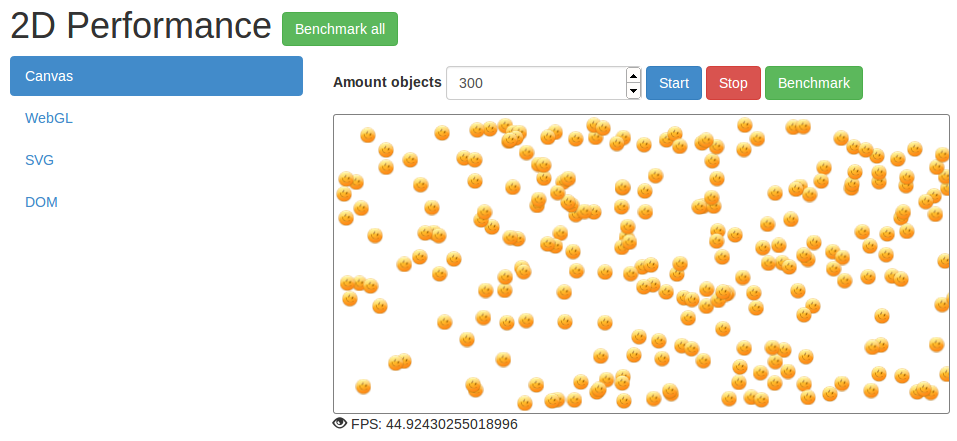
\includegraphics[width=\textwidth]{assets/demo_screenshot.png} 
	\end{center}
	\caption{Performance Messung}
	\label{performance_benchmark}
\end{figure}
\begin{figure}[h!]
	\inputminted{javascript}{assets/benchmark1.js}
	\caption{Spiele-Logik und Physik}
	\label{benchmark1}
	\newpage
\end{figure}
Außerdem kann per Klick der Benchmark-Wert für alle Technologien nacheinander ermittelt werden. Diese Tests werden dann auf möglichst vielen verschiedenen Geräten und Browsern durchgeführt. So entsteht eine gute Übersicht, was eine Technologie leisten kann.
\paragraph{Browser-Verlgeich} Für die Performance-Messungen in diesem Dokument wurde für jede Technologie der Benchmark in 3 Browsern durchlaufen: Firefox, Chrome und Internet Explorer. Dabei wurden die Tests auf meinem Mittelklasse-PC mit Windows 7 und aktuellen Grafiktreibern durchgeführt. Eine Grafik veranschaulicht jeweils die Ergebnisse.
%TODO: welche ie-version? vllt neue ausprobieren?
\newpage
\section{HTML5-Canvas}
\paragraph{} Eine tolle Möglichkeit, im Browser pixelgenaue Grafiken zu erzeugen, ist die HTML5 Canvas-API. Indem immer wieder eine Szene mit neuen Parametern gezeichnet wird, kann auf diese Weise ein 2D-Spiel programmiert werden.
\subsection{Technologie}
\paragraph{} Das Canvas-Element (englisch für Leinwand) und die entsprechende Javascript-API ist von der WHATWG-Arbeitsgruppe spezifiziert und wird von allen großen Browser-Herstellern implementiert. Dadurch ist gesichert, dass ein Browser-Spiel, das das Canvas-Element zur Darstellung nutzt, in auch vielfältigen  Umgebungen korrekt funktioniert. Auch WebGL gehört zum Canvas-Standard, da das Canvas-Element verschiedene Kontexte unterstützt; dieses Kapitel behandelt jedoch ausschließlich den \glqq 2d\grqq-Kontext, der \glqq webgl\grqq-Kontext wird im Kapitel \emph{WebGL} behandelt.
\paragraph{API} Die Canvas-API zeichnet sich besonders durch Schlichtheit und eine niedrige Lernkurve aus. Dabei ist der Zeichen-Kontext als Zustandsautomat implementiert, d.h. es werden nicht alle Informationen zum Zeichnen einer Linie in einem Methoden-Aufruf mitgegeben, sondern in mehreren. Erst wird der Zeichen-Stil konfiguriert, dann wird der Pfad definiert und dann die Linie gezeichnet.
\begin{figure}[h!]
	\begin{minted}{javascript}
	context.strokeStyle = '#fa00ff'; //definiere Farbe
	context.lineWidth = 5; //definiere Stift-Breite
	context.lineCap = 'round'; //definiere Linien-Abschluss
	context.beginPath(); //definiere pfad
	context.moveTo(0,0); //...
	context.lineTo(100,100); //...
	context.stroke(); //zeichne linie mit obigen einstellungen
	\end{minted}
	\caption{Canvas-Beispiel}
	\label{canvas-example}
\end{figure}
Da in der Praxis meist mehrere Zeichenoperationen mit der selben Konfiguration durchgeführt werden, hat dies den Vorteil dass so Rechenleistung gespart werden kann und der Quellcode einfacher bleibt.
\paragraph{Umfang} Mit dem Canvas-Element lassen sich unter anderem folgende Dinge zeichnen:
TODO: quote wikipedia here
\begin{itemize}
	\item Linien (gestrichelt, durchgezogen, ...)
	\item (gefüllte) Rechtecke
	\item Kreisbögen
	\item (gefüllte) Ellipsen
	\item Bezierkurven
	\item Gradienten
	\item Pixel-Grafiken (alles, was mit dem Image-Objekt geladen werden kann)
	\item Text
	\item Transparenz
\end{itemize}
Damit ist es perfekt geeignet, um auch aufwendige 2D-Spiele darzustellen, die meistens aus Serien von Pixelgrafiken bestehen, die in schneller Folge eingeblendet werden (sogenannte \emph{Sprites}).
\subsection{Unterstützung}
\begin{figure}[H]
	\begin{center}
		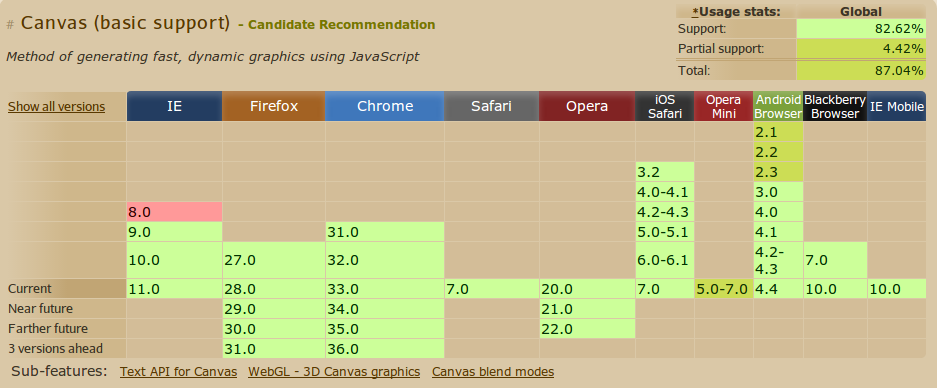
\includegraphics[width=\textwidth]{assets/canvas_support.png} 
	\end{center}
	\caption{Canvas Unterstützung}
	\label{canvas_support}
\end{figure}
Der 2D-Kontext wird von allen modernen Browsern unterstützt, Opera Mini bildet hier die einzige Ausnahme; sogar mobile Browser bieten die API durchgehend an. Sogar Internet-Explorer, der dafür bekannt ist, bei der Untersütztung von Standarts aus dem Rahmen zu fallen, bietet Canvas ab der Version 9.0 an. Natürlich gibt es viele Internet-Nutzer, die auch sehr alte Versionen von Browsern benutzen, allerdings sind diese für die Zielgruppe der online Spielenden Bevölkerung nicht besonders relevant; die meisten dieser alten Browser werden in Firmen mit veralteter IT-Technik benutzt, wo das Spielen am Computer sowieso verboten ist.
TODO: bild vom support einbinden.
\subsection{Bibliotheken}
Canvas ist die mit Abstand am weitesten verbreitete der hier vorgestellten Technologien. Dies ist wohl vor allem der niedrigen Lernkurve und dem schnellen Einstieg mit frühen Erfolgen zu danken. Daher ist die Community sehr aktiv und hat unzählige Tools, Bibliotheken und Frameworks entwickelt. Die wichtigsten dieser Tools werden hier in Kürze vorgestellt:
\subsubsection{KineticJS}
KineticJS ist eine auf HTML5 Canvas spezialisierte, quelloffene Bibliothek, d.h. sie bietet keinen Technologie-Fallback an. Sie abstrahiert die Canvas-API und bietet eine Objekt-Orientierte API an, in der \emph{Shapes} definiert werden, die zu Gruppen zusammengefasst werden und dann verschiedenen \emph{Layers} zugeordnet werden. Die Layer zusammen bilden den Szene-Graph
en, der alle dargestellten Objekte beinhaltet. Die einzelnen Objekte der Szene können jetzt unabhängig animiert und transformiert werden. Dabei ist nicht nur Rotation und Translation mö
glich, sondern z.b. auch Farb-Transformation u.Ä. Dazu kommt noch eine ereignis-basierte Architektur, mit der Animationen synchronisiert werden können.
\paragraph{Beispiel}
Anbei ein kleines Beispiel, wie der KintectJS-Code aussieht. In diesem Beispiel wird eine neue Szene (auch Stage genannt) angelegt und ein rotes Dreieck an einer zufälligen Position angezeigt.
\begin{figure}[h!]
	\inputminted{javascript}{assets/kineticjs_example.js}
	\caption{KineticJS Beispiel}
	\label{kineticjs_example}
\end{figure}
\paragraph{Verwendung} KineticJS wird bereits in vielen verschiedenen aktiven Projekten eingesetzt, auf http://kineticjs.com/ gibt es eine ganze Auswahl von verschiedenen Browser-Spielen, die mit dieser Bibliothek entwickelt wurden. Im Entwickler-Forum Stackoverflow gibt es hunderte Fragen zum Thema und über Google lassen sich Dutzende Tutorials finden, wie kleine Spie
le mit KineticJS entwickelt werden können.
\subsubsection{EaselJS}
EaselJS ist eine Bibliothek, deren API an Flash angelehnt ist. So fällt der Übergang leichter. Darüber hinaus existieren verschiedene Tools, die alle auf (ehemalige) Flash-Entwickler abzielen. Zum Beispiel gibt es EaselFL, ein Flash-Fallback für alte Browser, die Canvas nicht unterstützen, oder Zoe, ein Exporter für SWF-Animationen in EaselJS-Spritesheets.
\paragraph{TweenJS/SoundJS/PreloadJS} EaselJS kümmert sich nur um die reine Arbeit mit HTML5 Canvas, Funktionen wie Animationen und Transformationen oder Sounds sind in eigenen Modulen gekapselt:
\begin{itemize}
	\item \emph{TweenJS} für Animationen und Transformationen
	\item \emph{SoundJS} für Arbeiten mit Sounds
	\item \emph{PreloadJS} für das Managen und Laden von Bildern und Spiele-Inhalten
\end{itemize}
Damit ist die EaselJS-Suite nicht nur eine Bibliothek für das Arbeiten mit Canvas, sondern bietet Werkzeuge, um ganze Browser-Spiele oder andere Anwendungen zu entwickeln.
\subsection{Beispiel}
Wie bereits erwähnt, ist die API von Canvas sehr schlicht und einfach zu erlernen. Dabei spielt sich alles im sogenannten Context-Objekt ab. Auf diesem können Methoden aufgerufen werden, um Bilder oder Linien auf  die Arbeitsfläche zu zeichnen. Um Animationen oder ähnliches zu realisieren, empfiehlt es sich, die Methode requestAnimation-Frame zu verwenden.
\paragraph{requestAnimationFrame} Diese Methode bekommt als Parameter eine Funktion übergeben, die nach gewisser Zeit vom Browser aufgerufen wird. Üblicherweiße ruft diese Funktion rekursiv wieder requestAnimationFrame mit sich selbst als Parameter auf. Der Browser fungiert hier als Balancer und sorgt dafür, dass die Methode nicht öfter aufgerufen wird als nötig. So wird zum Beispiel die Framezahl pro Sekunde beschränkt und keine weiteren Aufrufe angefordert, wenn das Browser-Fenster nicht im Vordergrund ist. Um die Ablaufgeschwindigkeit des Spiels vom Verhalten der requestAnimationFrame-Methode zu entkoppeln, muss bei jedem Aufruf ermittelt werden, wie viel Zeit seit dem letzten Aufruf vergangen ist und zum Beispiel Bewegungs-Vektoren entsprechend angepasst werden.
\begin{figure}[H]
	\inputminted{javascript}{assets/vanillacanvas_example.js}
	\caption{Canvas-Beispiel}
	\label{canvas_support2}
\end{figure}
\subsection{Performance}
Mithilfe des oben erwähnten Benchmark-Tests wurden auf einem Desktop-Rechner 8500, auf einem Smartphone 230 und auf einem Macbook 4000 Objekte simultan bei 30FPS dargestellt. Damit ist Canvas auf jeden Fall geeignet, um auch komplexe Browser-Spiele für PCs und Laptops zu entwickeln. Einfache Spiele mit nur wenig Polygonen dürften auch auf Handys kein Problem sein. Allerdings ist die Zeichengeschwindigkeit auf dem Smartphone auch nicht konstant, sonder fällt manchmal stark ab. Für grafikgewaltige Handyspiele, die es mit nativen Apps bereits gibt, ist Canvas-HTML5 sicherlich nicht geeignet.
\paragraph{Verbesserungen} Zu beachten ist, dass meine Implementierung einer Canvas-Renderfunktion recht naiv war. Es ist sicherlich möglich, hier durch verschiedene Tricks mehr Performance zu erreichen, größere Spiele lassen sich dadurch aber trotzdem nicht relasieren. Im folgenden sind verschiedene Techniken vorgestellt, um die Performance von Canvas-Spielen zu verbessern.
\paragraph{Pre-Rendering in unsichtbares Canvas} Eine gängige Technik ist es, z.B. eine komplexe Hintergrund-Szenerie, die sich jeoch selten ändert, einmal zu rendern und in einem unsichtbaren zweiten Canvas-Element zwischenzuspeichern. Das Bild kann dann für jeden Frame in das sichtbare Canvas kopiert werden, was sehr effizient möglich ist.
\paragraph{Neuzeichnen von Bereichen} Bei manchen Anwendungen ändert sich nicht bei jedem neuen Frame der gesamte Bildschirm, sondern nur ein kleiner Teilausschnitt (ein Ball bewegt sich über ein statisches Spielfeld). Hier wäre es möglich, nur den Teil des Canvas neu zu zeichnen, der sich auch tatsächlich verändert hat.
\paragraph{Konfiguration des Zeichenautomaten nur ändern wenn nötig} Wie bereits im Kapitel \emph{API} vorgestellt, ist es möglich den Zeichenmodus einmal festzulegen und dann gleiche Zeichenoperationen durchzuführen. So ist es zum Beispiel deutlich performanter, erst alle gestrichelten Linien und dann alle durchgezogenen Linien in einer Szenerie zu zeichnen als immer abwechselnd, da so das Canvas-Element intern Optimierungen durchführen kann.
\paragraph{Rechenaufwändige Effekte vermeiden} Built-In-Effekte wie weicher Schatten sind zwar sehr bequem zu verwenden, benötigen aber viel Rechenzeit. Am besten ist aus, auf solche Effekte ganz zu verzichten oder mit halb-transparenten Grafiken zu arbeiten.
\paragraph{Ganzzahlige Koordinaten verwenden} Das Canvas-Element unterstützt zwar Subpixel-Rendering, allerdings sind diese sehr ineffizient, da die Farbe eines Pixels erst kompliziert berechnet werden muss. Verwendet man nur ganze Zahlen als Koordinaten besonders für Bilder, können die Pixel direkt eingefügt werden und es wird kostbare Ausführungszeit gespart.
\newpage
\subsubsection{Browser-Vergleich} Beim Test des Canvas-Benchmarks in verschiedenen Browsern stach vor allem Firefox hervor. Leider konnte auch nach Recherche kein wirklicher Grund für diese Performance gefunden werden; in der Vergangenheit kam es des öfteren bei verschiedenen Browsern zu massiven Performance-Einbrüchen nach dem Update auf eine bestimmte Version. Möglich, dass Chrome und der Internet-Explorer hier Konfigurations-Probleme haben oder die Grafik-Karte im Test nicht richtig unterstützen.
Sowohl die großen Differenzen der Performance verschiedener Browser als auch der Fakt, dass die Performance nach bestimmten Updates plötzlich stark abnimmt und sich mit dem nächsten Update wieder normalisiert, ist es Zeichen dafür, dass die Technologie selbst, obwohl schon einige Jahre alt, noch nicht hunderprozentig stabil läuft. Die Browser-Hersteller sind immer noch am optimieren und verbessern der ihrer Implementierungen. Über die verschiedenen Versionen hinweg zeichnet sich jedoch ein deutlicher Trend nach oben ab.
\paragraph{Kleine Stichprobe} Zu beachten ist ebenfalls, dass die im Benchmark verwendete Methode (Zeichnen eines Bildes) zwar in so gut wie jedem 2D-Spiel verwendet werden dürfte, aber höchstwahrscheinlich nicht so ausschließlich wie hier. In der Praxis können sich daher andere Flaschenhälse ergeben, die die Performance eines gewissen Spiels in einer gewissen Version eines gewissen Browsers beeinflussen, oder eventuelle Flaschenhälse im Benchmark-Beispiel werden umgangen. Durch diese Effekte kann sich das Verhältnis der Browser deutlich verschieben, trotzdem bietet der Benchmark eine gute Orientierung, da wie bereits erwähnt eine essentielle Funktion der API genutzt wird.
%TODO: checken, ob chrome durch config schneller wird
\begin{figure}[H]
	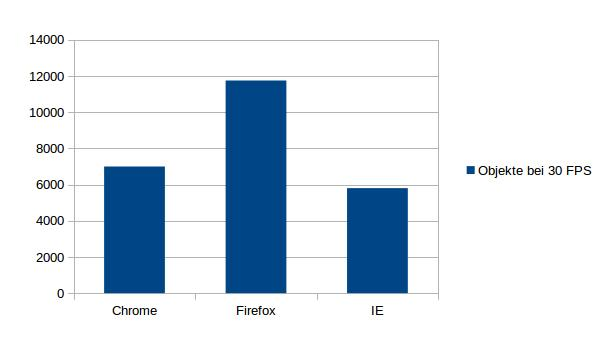
\includegraphics[width=\textwidth]{assets/browser_comp_canvas} 
	\caption{Browser-Vergleich Canvas}
	\label{browser_comp_canvas}
\end{figure}
\newpage
\section{WebGL}
Einen ganz anderen als Canvas verfolgt die Technologie WebGL. Hier wird nicht eine ganz neue API definiert, sondern die bereits bekannte API von OpelGL im Browser zu Verfügung gestellt.
\subsection{Technologie}
Genau wie HTML5-Canvas ist auch WebGL von der Khronos Group spezifiziert und wird über den <canvas>-Tag ins Dokument eingebunden. Der Unterschied besteht darin, dass nicht das \emph{2d}-Kontext-Objekt, sonder das \emph{webgl}-Kontext-Objekt genutzt wird. Dieses stellt die (recht umfangreiche) API zur Verfügung, um mit WebGL zu arbeiten. Im Gegensatz zu Canvas, dessen API auf Schlichtheit und eine niedrige Lernkurve abzielt, bringt WebGL im Grunde die gesamte OpenGL-Bibliothek in den Browser. Dabei steht nicht eine schlanke API, sondern Performance im Vordergrund.
\paragraph{3D oder 2D?} Entgegen der landläufigen Meinung ist WebGL \emph{keine} 3D-API, sondern unterstützt von Haus aus nur 2D-Zeichnungen. Allerdings ist es möglich, die 3D-Fähigkeit nachzurüsten und dabei trotzdem hochperformant zu bleiben, indem dieser Code direkt in GLSL implementiert werden kann
\paragraph{Nativer Shader-Code} Die \emph{OpenGL Shading Language} ist eine an C angelehnte Sprache, um Programme zu schreiben, die direkt auf der Grafikkarte ausgeführt werden. Sie dienen zum Beispiel dazu, die Position von Objekten im dreidimensionalen Raum zu berechnen oder die Farbe oder Textur eines Objektes zu bestimmen. Auch in WebGL können solche GLSL-Shader geschrieben und direkt im Browser kompiliert werden. So können Grafikberechnungen auf der Grafikkarte hoch-parallelisiert ausgeführt werden, was für die enorme Performance von WebGL im Vergleich zu anderen Technologien verantwortlich ist. Hier im Shader-Code würde man die Logik für das Umrechnen von 3D-Objekte in 2D-Objekte vornhemen.
\paragraph{Komplexe API} Dass WebGL so effizient arbeiten kann, muss der Entwickler einige Kompromisse eingehen. Die auf dem Gebiet der 3D-Spieleentwicklung für Desktop-PCs unerfahrenen Entwickler werden die API sicherlich als unintuitiv und sperrig empfinden. So müssen zum Zeichnen eines einfachen Quadrats folgende Schritte durchgeführt werden:
\begin{itemize}
	\item Vertex-Shader schreiben (Umrechung der Koordinaten)
	\item Fragment-Shader schreiben (Erzeugen von Textur oder Farbe)
	\item Shader kompilieren und linken
	\item Daten-Buffer an Attribut für den Shader binden
	\item Daten-Buffer mit Koordinaten für 2 Dreieicke füllen
	\item bei Textur: Textur-Koordinaten-Buffer an Attribut für den Shader binden und füllen (auch hier für Dreieicke)
	\item Dreiecke zeichnen
\end{itemize}
In der Praxis macht es Sinn, ein anstrahierendes Framework zu nutzen, dass man sich nicht mehr direkt mit der sperrigen WebGL-API auseinandersetzen muss. Allerdings sind dann auch keine Low-Level-Optimierungen möglich, die das Programm teilweise dramatisch beschleunigen können.
Im Vergleich zur Canvas-API muss hier also viel Vorarbeit geleistet werden, bevor Resultate zu sehen sind.
\paragraph{Canvas/WebGL-Hybrid} Mit WebGL sind zwar viele Dinge möglich, allerdings bietet es nur eine Low-Level-API. Zum Beispiel ist in der WebGL-Spezifikation kein nativer Text-Renderer vorgesehen. Natürlich ist es möglich, sich selbst einen Shader für diesen Zweck zu schreiben, allerdings gibt es die viel einfachere Lösung, gebrauch von der High-Level-API des Canvas-Elements zu machen und den Text in einem versteckten HTML5-Canvas zu rendern. Der Inhalt dieses Canvas kann dann als Textur in den WebGL-Kontext eingebunden und genutzt werden. Dies kann zum Beispiel im Lade-Zyklus des Spiels einmalig durchgeführt werden. So hat man alle Funktionen von HTML5-Canvas zur Verfügung, kann aber trotzdem von der gewaltigen Performance von WebGL Gebrauch machen.
\paragraph{Rechteck-Koordianten} Um zum Beispiel ein Rechteck zu zeichnen, muss beachtet werden, dass die Koordinaten in WebGL nicht Pixeln entsprechen; es werden sogenannte Clipspace-Koordianten verwendet. Dabei ist die linke untere Ecke der Zeichenfläche immer -1 -1 und die rechte obere Ecke immer 1 1. In realen Anwendungen übernimmt die Umrechnung von Pixel- in Clipspace-Koordianten meist der Shader selbst - er benötigt dafür lediglich die Größe der Zeichenfläche in Pixeln. Die andere Besonderheit ist, dass nicht nur 4 Vertizes übergeben werden, wie man für ein Rechteck annehmen würde, sondern 6. Das liegt daran, dass in WebGL immer Dreiecke gezeichnet werden, daher müssen 2 Punkte doppelt definiert werden. Außer dem Zeichenmodus Dreiecke gibt es noch Spezialfälle, bei denen Vertizes eingespart werden können, diese würden jedoch diesen Rahmen sprengen.
\newpage
\subsection{Pixi.js} Anders als die bisher vorgestellten Frameworks ist Pixi.js nicht nur ein vereinfachender API-Wrapper für die Zeichen-Technologie selbst, sondern eine komplette Game-Engine, bei der zwar der Haupt-Augenmerk auf dem Renderer liegt, aber viele andere Funktionen wie Kollisions-Erkennung, Multi-Plattform-Support (Mobile, PC), Multi-Touch, ein Asset-Loader und vieles mehr eingebaut sind. Dieser Abschnitt befasst sich aber hauptsächlich mit dem eingebauten Renderer.
\paragraph{Canvas-Fallback} Der Pixi.js-Renderer untersützt sowohl WebGL als auch Canvas; falls möglich, wird WebGL genutzt. So soll schlicht die Reichweite der pixi.js-Spiele erhöht werden, da viele Geräte in Umlauf zwar eine rudimentäre Canvas-Unterstützung, aber noch keinen Support für WebGL haben.
\paragraph{Text-Rendering} Der oben erklärte Trick, die Canvas-API zu nutzen, um Text in Bitmap-Texturen für WebGL umzuwandeln, wird auch von pixi.js genutzt.
\paragraph{Beispiel}
Da Pixi.js eine komplette Game-Engine ist, ist die API sehr abstrakt gehalten - man steuert \emph{Game-Objects} und Viewports, das wirkliche Zeichnen in das Browser-Fenster spielt eine untergeordnete Rolle. Zum ausbalancieren der Game-Ticks wird auch hier die Methode requestAnimationFrame genutzt.  Im folgenden Beispiel wird eine Pixi-Szene mit Renderer intialisiert und ein neues Objekt in die Szene gesetzt. Dieses Objekt wird dann bei jedem Game-Tick ein Stückchen weiter rotiert.
\begin{figure}[H]
	\begin{minted}{javascript}
var stage = new PIXI.Stage(0x66FF99);
var renderer = PIXI.autoDetectRenderer(400, 300);
document.body.appendChild(renderer.view);
requestAnimFrame( animate );
var texture = PIXI.Texture.fromImage("bunny.png");
var bunny = new PIXI.Sprite(texture);
bunny.anchor.x = bunny.anchor.y = 0.5;
bunny.position.x = bunny.position.y = 150;
stage.addChild(bunny);
function animate() {
    requestAnimFrame( animate );
    bunny.rotation += 0.1;
    renderer.render(stage);
}
    \end{minted}
    \caption{pixi.js Beispiel}
    \label{pixijs_example}
\end{figure}
\newpage
\subsection{Beispiel}
%http://www.html5rocks.com/en/tutorials/webgl/webgl_fundamentals/ zitieren
Da die WebGL-API recht komplex ist, kann aufgrund des Umfangs nur ein kleines Beispiel gezeigt werden. Der folgende Code zeichnet ein grünes Rechteck über die gesamte Größe der Zeichenfläche. Dafür müssen die unten definierten Shader für Farbe und Position kompiliert und gelinkt werden, dann müssen die Koordinaten für das Rechteck dem Shader als \emph{Buffer} übergeben werden.
\begin{figure}[H]
	\inputminted{javascript}{assets/vanillawebgl_example.js}
	\caption{WebGL-Beispiel}
	\label{webgl_example}
\end{figure}
\newpage
\subsection{Performance}
Die Anzahl der darzustellenden Objekte mit WebGL übertrifft die der anderen Technologien um Weiten. Selbst mit einem Smartphone sind über 10.000 Objekte bei 30FPS möglich, bei einem Computer mit dedizierter Grafikkarte sogar über 80.000. Diese enormen Zahlen sind möglich, da bei WebGL keine Abstraktions-Schichten zwischen der Grafikkarte und den Javascript-Zeichenbefehlen liegen. Die Instruktionen werden direkt an die Grafikkarte durchgereicht und dort ausgeführt, was aufgrund der parallelen Verarbeitung extrem schnell geschieht. Natürlich sind die oben genannten Werte nur durch Optimierungen im Zusammenspiel zwischen Javascript und Grafikkarte möglich.
\paragraph{Textur-Caching} Der im Kapitel Performance-Messung definierte Benchmark-Test setzt einige Vorraussetzungen, die weitreichende Optimierungen ermöglichen. Zum einen gibt es nur eine Pixelgrafik, also eine Textur, die in der Szene dargestellt wird, zum anderen verändern die Objekte zwar ihre Position, nicht jedoch ihre Anzahl oder Rotation. Dies ermöglicht es unter anderem, die Bitmap-Grafik für die Textur einmal in den Grafikspeicher zu laden und dann immer wieder aufzurufen. In einem echten Spiel, in dem viele verschiedene Grafiken benötigt werden, ist es gut möglich, dass selten genutzte Grafiken ab und zu aus dem Arbeitsspeicher der Grafikkarte verdrängt werden und dann neu aus dem Hauptspeicher geladen werden müssen, was einen Performance-Abbruch zur Folge hätte.
Dadurch, dass die Anzahl der Objekte immer konstant bleibt, ist ein statischer Puffer für die Textur-Koordinaten völlig ausreichend - dieser muss zu Beginn einmal befüllt werden und kann dann im Grafikspeicher verbleiben.
\paragraph{Effizienter Shader} Der Shader-Code wird für jeden Frame, den die Grafikkarte an den Bildschirm weitergibt, tausende Male aufgerufen. Zwar wird dieser in nativen Op-Code kompiliert und somit sehr effizient durchgeführt, dennoch ist es empfehlenswert, hier möglichst sparsam mit den Resourcen den Grafikkarte umzugehen und keine komplizierten Berechnungen durchzuführen. Im Benchmark-Test gibt es keine Rotation oder ähnliches, also müssen die Pixel-Koordinaten nur in Clipspace-Koordinaten von -1 bis 1 umgerechnet werden und rechenaufwändige Operationen wie Sinus werden gespart.
\paragraph{Batch-Verarbeitung} Der Flaschenhals bei der Verwendung von WebGL ist die Datenübertragung aus dem JavaScript-Kontext in den Speicher der Grafikkarte. Daher lohnt es sich, die Koordinaten für das Zeichnen von gleichartigen Objekten alle gleichzeitig in den Grafikspeicher zu übertragen, um dann alle Objekte auf einmal zeichnen zu lassen, statt für jedes Objekt den Kontext zu wechseln; also die Koordinaten eines Objekts zu übertragen, das Objekt zeichnen lassen, und dann die Koordianten des nächsten Objekts zu übertragen. In der WebGL-Implementierung des Benchmark-Tests explodierte die Anzahl der gezeichneten Objekte bei 30FPS von knapp 4.000 auf über 80.000. Um die Performance-Vorteile von WebGL nutzen zu können, muss diese Optimierung also unbedingt ausgeführt werden, wie zum Beispiel im pixi.js-Framework.
\paragraph{Treiber-Probleme} In ungünstigen Situationen kann WebGL eine sehr schlechte Performance liefern, obwohl die oben genannten Optimierungen angewand wurden. Ursache ist in vielen Fällen die fehlende Unterstützung der WebGL-Implementierung für die im Rechner verbaute Grafikkarte. Hier empfiehlt es sich, die Grafik-Treiber und den Browser immer aktuell zu halten.
\paragraph{Performance-Bremsen} Gerade in Chrome sind standardmäßig viele Einstellungen aktiviert, die in gewissen Konstellationen von Browser, Betriebssystem und Hardware zu Problemen führen können. Leider ist es als Entwickler kaum möglich, Abhilfe für diese Probleme zu schaffen, es muss jedoch bei der Programmierung bewusst sein, dass die Performance auf dem Entwicklungs-Rechner bei gewissen Kunden nicht erreicht werden kann.
\paragraph{Dataflow} Bei der Optimierung von WebGL-Anwendungen ist es wichtig, zu verstehen, wie eine GPU arbeitet. Eine GPU verarbeitet einen Strom von Daten - am effizientesten ist es, diesen Strom so selten wie möglich zu unterbrechen oder zu verlangsamen. Zum Beispiel benötigt der Upload einer Textur in den Grafikspeicher einige Zeit. Wenn also direkt nach einem Textur-Upload ein Zeichenbefehl für diese Textur übetragen wird, blockiert die GPU, bis die Textur vollständig gelesen wird. Also sollten zuerst andere Zeichen-Operationen durchgeführt werden, bis die Textur vollständig geladen ist. Ein anderes Beispiel sind sogenannte \emph{Readbacks}, bei denen Daten von der GPU zurück in den JavaScript-Kontext geladen werden. Für diese Operation muss die JavaScript-Ausführung blockiert werden, bis die GPU die Daten geliefert hat. In dieser Zeit können keine Zeichen-Operationen von JavaScript and die Grafikkarte übermittelt werden und der Daten-Strom setzt aus. Daher sollten Readbacks soweit wie möglich vermieden werden.
\paragraph{Ausblick} Da durch WebGL alle Fähigkeiten einer Grafikkarte in JavaScript offen gelegt werden, ist eine sehr genaue Steuerung und damit auch Optimierung des Zeichenprozesses möglich. Diese genau zu erklären, würde den Rahmen in dieser Ausarbeitung sprengen. Zusammenfassend lässt sich sagen, dass WebGL zwar kompliziert und die dahinterstehenden Konzepte umfangreich und schwierig zu verstehen sind, die Technologie selbst aber dadurch in Sachen Performance den anderen vorgestellten Technologien deutlich überlegen ist. 
%TODO: quote https://docs.google.com/presentation/d/12AGAUmElB0oOBgbEEBfhABkIMCL3CUX7kdAPLuwZ964
\newpage
\subsubsection{Browser-Vergleich} Beim Vergleich der 3 wichtigsten Browser fallen sowohl die sehr hohe Performance von Chrome als auch die recht schwache Performance des Internet-Explorer ins Auge. Das Problem in Internet-Explorer ist höchstwahrscheinlich eine fehlende Unterstützung der Grafikkarte - dadurch muss die Berechnung der Vertizes usw. in der CPU ablaufen und alle Vorteile von WebGL können nicht ausgespielt werden. Chrome hat hier eine deutlich bessere Anbindung an die Grafikkarte; dadurch kann die Berechnung hoch-parallelisiert ablaufen und eine sehr hohe Objekt-Zahl erreicht werden.
%TODO: quote https://www.scirra.com/blog/125/internet-explorer-11-webgl-and-more
\paragraph{Widersprüchliche Ergebnisse} In einem Benchmark-Test der Website scirra.com zeichnet sich ein ganz anderes Bild. Hier kann der Internet Explorer 11 deutlich mehr Objekte zeichnen als Chrome oder Firefox. Auch das weisst darauf hin, dass in meinem Test der Internet Explorer die große Rechenleistung der Grafikkarte aus unbekannten Gründen, höchstwahrscheinlich Treiberproblemen, nicht nutzen kann. Daraus wird ersichtlich, dass Benchmarks mit kleinen, dedizierten Beispielen auf nur wenigen Plattformen äußerst missverständlich sein können; es wird hier keine Aussage darüber getroffen, dass Internet Explorer eine schlechtere Performance liefert als Chrome, sondern dass durch viele Abstraktionsschichten zwischen Hardware und Software sehr große Differenzen auftreten können, auch wenn die theoretisch mögliche Performance identisch ist.
\begin{figure}[H]
	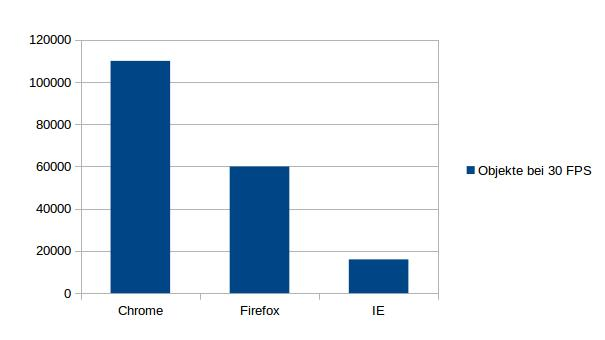
\includegraphics[width=\textwidth]{assets/browser_comp_webgl} 
	\caption{Browser-Vergleich WebGL}
	\label{browser_comp_webgl}
\end{figure}
\newpage
\section{SVG}
Anders als WebGL oder Canvas ist SVG deklarativ, d.h. es wird kein Befehl gegeben, ein Rechteck zu zeichnen, sondern es wird ein Rechteck-Element mit gewissen Parametern definiert, welches dann vom System automatisch gezeichnet wird. Eine pixelgenaue Kontrolle ist hier nur sehr schwer nötig, dennoch ist die SVG-Technologie sehr interessant, auch für Browser-Spiele.
\subsection{Technologie}
SVG (Scalable Vector Graphics) ist eine vom W3C entwickelte Spezifikation für eine XML-basierte Sprache zur Beschreibung von 2-dimensionalen Vektorgrafiken. Dabei handelt es sich um eine deklarative Beschreibung, das heißt, Interaktivität oder Animationen müssen von aussen gesteuert werden (zum Beispiel über JavaScript).
\paragraph{SMIL} Es ist auch möglich, SVG-Animationen mit SMIL (Synchronized Multimedia Integration Language) zu beschreiben, das ebenfalls auf XML basiert. Allerdings eignet sich diese Sprache eher für statische Animations-Abläufe (Filme etc.) und ist für echtzeit-dynamische Browserspiele ungeeignet. Aus diesem Grund wird in diesem Dokument nicht tiefer darauf eingegangen.
\paragraph{Integration} Alle modernen Browser unterstützen von Haus aus SVG, entweder in einer separaten .svg-Datei oder, für die Spiele-Entwicklung interessanter, direkt in das HTML der Website eingebettet. Mit den herkömmlichen JavaScript-APIs für den DOM-Zugriff lässt sich auch SVG steuern. Dabei muss beim Erstellen der SVG-Elemente nur der korrekte XML-Namespace angegeben werden.
\begin{figure}[h!]
	\inputminted{javascript}{assets/svg_example.js}
	\caption{SVG Namespace-Elemente}
	\label{svg_namespace_example}
\end{figure}
Wie im Beispiel \emph{SVG Namespace-Elemente} gut erkenntlich ist, macht es von JavaScript-Seite keinen Unterschied, ob es sich um ein herkömmliches DOM-Element oder ein SVG-Element handelt, die API mit Methoden wie createElement oder appendChild bleibt die gleiche.
\paragraph{Umfang} Die SVG-API ist recht umfänglich, d.h. es müssen nicht grunsätzliche Funktionen wie Text-Rendering selbst implementiert werden. Zu den Fähigkeiten von SVG gehören das Darstellen von Polygonen, Kreisen und Rechtecken als auch Texte und eingebundene Rastergrafiken.
\paragraph{Animation mit JavaScript} Da, wie bereits erwähnt, die Animationen in Spielen hoch dynamisch sind und ständig angepasst werden müssen, ist die einfachste Methode, SVG-Grafiken mit JavaScript zu animieren, die ständige Anpassung der Transformations-Parameter der einzelnen Elemente (Position, Drehung, ...). Deklarative Ansätze wie CSS3-Keyframe-Animationen oder SMIL eigenen sich höchstens für sich monoton wiederholende Hintergründe, nicht aber für Echtzeit-Spiele. Auch hier kann die HTML5-Methode \emph{requestAnimationFrame} genutzt werden, um eine sinnvolle Anpassungsrate des SVG-Dokuments zu gewährleisten.
\subsection{RaphaelJS}
RaphaelJS ist eine Abstraktions-Schicht für die SVG-API. Dabei wird ein \emph{Wrapper} sowohl für die SVG-Zeichenfunktionen als auch für die HTML-Eventhandler geboten. Hinzu kommen viele Hilfsmethoden, die das Erstellen von komplexen Grafiken deutlich beschleunigen. Vor allem für die Erstellung von Animationen aller Art ist die JavaScript-API von RaphaelJS sehr praktisch, da die XML-Animations-Notation in SVG sehr umständlich und schlecht lesbar ist.
\paragraph{Kompatibilität} Ein weiterer Vorteil von RaphaelJS ist die eingebaute Unterstützung für ältere Browser; für frühere Versionen des Internet-Explorers wird ein Fallback auf \emph{VML} durchgeführt.
\paragraph{Verwendung} RaphaelJS wird genau wie SVG selbst meistens für Diagramme und ähnliche, statische Zwecke eingesetzt, es gibt aber auch ein auf RaphaelJS basierendes Browserspiel, dass die Technik erfolgreich einsetzt: https://github.com/petehamilton/gravitas
\paragraph{Beispiel}
Wie im Beispiel zu sehen ist, muss man sich bei RaphaelJS an keiner Stelle mit Dingen wie HTML-Elementen oder SVG-Namespaces auseinandersetzen - RaphaelJS kapselt den Zugriff auf den DOM und bietet eine saubere, verständliche und leicht zu nutzende API an, für die die Programmier-Sprache nicht gewechselt werden muss. 
\begin{figure}[H]
	\begin{minted}{javascript}
// Creates canvas 320 x 200 at 10, 50
var paper = Raphael(10, 50, 320, 200);

// Creates circle at x = 50, y = 40, with radius 10
var circle = paper.circle(50, 40, 10);
// Sets the fill attribute of the circle to red (#f00)
circle.attr("fill", "#f00");

// Sets the stroke attribute of the circle to white
circle.attr("stroke", "#fff");	
	\end{minted}
	\caption{RaphaelJS Beispiel}
	\label{raphaeljs_example}
\end{figure}
\newpage
\subsection{Beispiel}
Das Arbeiten mit SVG ist sehr einfach, es muss nur für jedes Objekt im Spiel ein SVG-Element angelegt und dem Zeichenflächen-Element angehängt werden. Um z.B. die Position zu verändern, müssen nur die entsprechenden Attribute im SVG-Element gesetzt werden, in diesem Fall \emph{x} und \emph{y}. Zu beachten ist, dass es sich hierbei um die naive Implementierung handelt, die nicht auf die erweiterten Animations-Möglichkeiten von SVG zurückgreift. Dies ist in realen Anwendung auch oft gar nicht möglich, da jetzt die Animation in einer Sekunde noch gar nicht bekannt ist.

Wie bei jeder Technologie kann auch hier die Helfer-Methode \emph{requestAnimationFrame} verwendet werden, um die Anzahl der Renderings pro Sekunde konstant auf einem sinnvollen Level zu halten.

\paragraph{Namespaces} Die Namespaces in SVG sind umständlich zu programmieren, da man sie bei jeder Erstellung eines Elements und bei jedem Setzen eines Attributs der jeweilige Namespace angegeben werden muss; zusätzlich muss der Namespace noch mit Doppelpunkt getrennt vor den Attribut-Namen gesetzt werden. Weiter verkompliziert wird die Arbeit mit der SVG-API auch dadurch, dass beispielsweise das Attribut zum Setzen einer Rastergrafik als Hintergrund eines SVG-Objektes einen anderen Namespace hat als das SVG-Element selbst, die Koordinaten-Angaben dagegen haben gar keinen Namespace. Diesen Mehraufwand spart man sich am Besten durch die Verwendung einer Bibliothek, die diese Dinge gegenüber dem Programmierer abstrahiert.
\begin{figure}[H]
	\inputminted{javascript}{assets/vanillasvg_example.js}
	\caption{SVG-Beispiel}
	\label{svg_example}
\end{figure}
\newpage
\subsection{Performance}
%http://smus.com/canvas-vs-svg-performance/
Im Benchmark-Test schaffte die SVG-Implementierung nur 500 Objekte, wo WebGL 80.000 bzw. Canvas 9.000 rendern konnte. Das macht klar, dass SVG ungeeignet ist für Spiele mit vielen Objekten, die ständig neu gezeichnet werden müssen. Dennoch gibt es Spiele wie das oben erwähnte Gravitas, die erfolgreich SVG zur Darstellung einsetzen. Das hat vor allem damit zu tun, dass es auch im Spiele-Umfeld Anwendungen gibt, bei denen nur wenige Objekte gleichzeitig dargestellt werden, bzw. bei denen nur selten Neu-Zeichnungen durchgeführt werden. Ausserhalb des Spiele-Usecases eignet sich SVG daher vor allem für Statistiken oder Karten-Darstellungen. Ein Performance-Gewinn in SVG-Spielen ist vor allem dadurch möglich, das Neu-Zeichnen der kompletten Fläche zu verhindern und den Szene-Graph wie auch die Transformations-Anweisungen so aufzubauen, dass Optimierungen angewendet werden können. Wie bereits erwähnt ist die sorgfältige Definition von gleichmäßigen Bewegungen z.B. in einem Spiel wie Super-Mario, in dem sich Bewegungsrichtung und -art von Objekten ständig innerhalb von Sekunden ändert, nicht möglich.
\subsubsection{Browser-Vergleich} Im direkten Browser-Vergleich sticht die schlechte Unterstützung von Firefox ins Auge. Diese scheint ab Version 18 aufzutreten. Leider ist es sehr schwierig, hierfür die Ursache zu finden; die Browser entwickeln sich in enorm hohen Tempo weiter und Dinge wie die Performance für gewisse Operationen können von Version zu Version sehr stark fluktuieren.
\begin{figure}[H]
	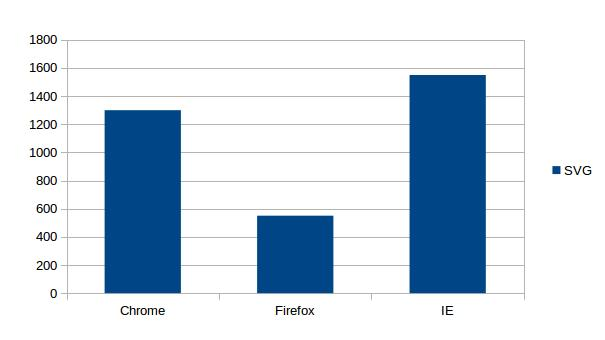
\includegraphics[width=\textwidth]{assets/browser_comp_svg} 
	\caption{Browser-Vergleich SVG}
	\label{browser_comp_svg}
\end{figure}
\newpage
\section{DOM}
2D-Spiele mit HTML, also dem Document-Object-Model (kurz DOM) darzustellen, funktioniert ganz ähnlich wie bei SVG. Durch die modernen CSS-Spezifikationen, die viele komplexe Effekte bereitstellen, ergeben sich dabei jedoch ganz andere Möglichkeiten.
\subsection{Technologie}
Eine andere Möglichkeit, HTML-Elemente zur Darstellung von Spiele-Objekten zu verwenden ist natürlich die Verwendung der Standard-HTML-Elemente in Verbindung mit CSS-Styling.
\paragraph{Support} Der größte Vorteil bei dieser Herangehensweise ist natürlich der in jedem Browser verfügbare Support. Wenn man sich für das Spiel auf einfache Rastergrafiken beschränkt und auf Rotation und ähnliches verzichtet, ist sogar CSS1 ausreichend. Allerdings untersützen alle modernen Browser CSS3 - dadurch sind auch Dinge wie Rotationen, einfache Filter, 3D-Transformationen, Schatten und viele andere Dinge möglich. Abbildung \ref{css_transforms_support} zeigt die Browser-Unterstützung für CSS-Transforms. Dazu gehören Rotationen, Skalierungen und freie Matrix-Transformationen. 
\begin{figure}[H]
	\begin{center}
		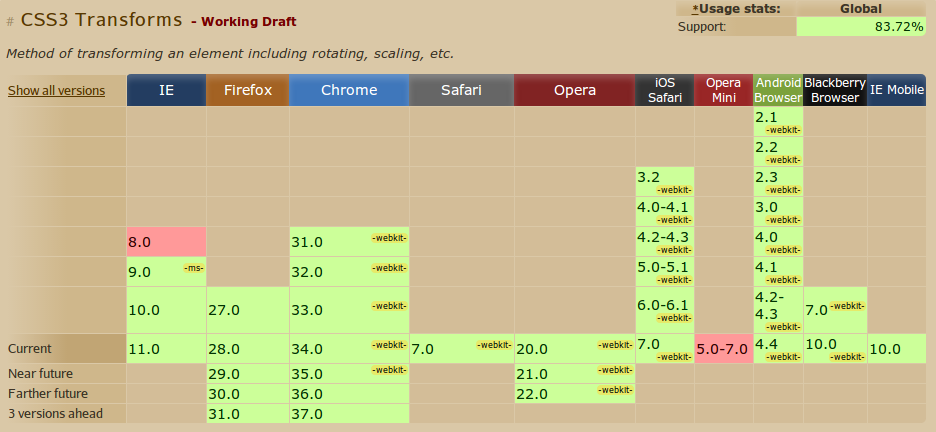
\includegraphics[width=\textwidth]{assets/css_transforms_support.png} 
	\end{center}
	\caption{CSS3-Transforms Unterstützung}
	\label{css_transforms_support}
\end{figure}
\paragraph{CSS Hardware-Unterstützung} CSS3-Transformationen werden in vielen modernen Browsern mit \emph{Hardware-Unterstützung}, also mithilfe der Grafikkarte berechnet. Das beschleunigt rechenaufwändige Effekte wie Schatten oder 3D-Transformationen enorm.
\paragraph{Interaktivität} Da Spiele-Objekte hier auch DOM-Elemente sind, ist es problemlos möglich, Events wie Klick oder Mouse-Over zu binden und für die Interaktivität im Spiel zu nutzen. Bei Canvas oder WebGL beispielweise muss selbst berechnet werden, wann und ob solche Ereignisse eintreten.
\subsection{Sprite.js}
Das Framework  Sprite.js, das sich darauf spezialisiert hat, Sprites, also Animationen mit Einzelbildern für jeden Frame, in jedem Browser darzustellen, hat sowohl einen Renderer für Canvas, WebGL als auch DOM-Elemente. Das Augenmerk liegt hier vor allem an der Portabilität; die Darstellung von Sprites als DOM-Element beherrscht jeder Browser. Der Vorteil des Frameworks ist es, dass eine Abstraktions-Schicht gegeben ist, mit der sowohl DOM als auch WebGL und Canvas mit der selben, einfach zu erlernenden API gesteuert werden können.
\paragraph{Verwendung} Verschiedene kleine Browsergames wie Steam oder Webbattle.js setzen Sprite.js ein, eine richtige Community hat sich jedoch bisher nicht gebildet. Generell wird das Thema Browser-Spiele mithilfe des DOM innerhalb der Web-Community eher selten angegangen.
%http://batiste.dosimple.ch/games/steam9/
% https://github.com/tadast/webattle.js
\subsection{Beispiel}
Die Arbeit mit herkömmlichen DOM-Elementen gleicht dem Ansatz von SVG stark. Es ist sogar noch einfacher, die Elemente anzuzeigen, da auf Namespaces usw. verzichtet werden kann. Genau wie bei SVG wurde eine naive Implementierung verwendet, die einfach die Position der Spiele-Objekte bei jedem Game-Tick neu setzt, was in vielen realen Spiele-Anwendungen nötig sein würde.
\begin{figure}[H]
	\inputminted{javascript}{assets/vanilladom_example.js}
	\caption{DOM-Beispiel}
	\label{dom_example}
\end{figure}
\newpage
\subsection{Performance}
Die DOM-Implementierung schafft je nach Browser zwischen 450 und 500 Objekten, wenn Canvas 9.000 oder WebGL 80.000 schafft. Damit rangiert sie noch knapp unter der Performance von SVG und ist wie SVG selbst nicht geeignet, schnelle, interaktive Spiele darzustellen. Jedoch wurde auch hier genau wie bei SVG auf die Verwendung von CSS-Transitionen oder ähnliches verzichtet, was bei gleichförmigen Bewegungen auf jeden Fall einen Performance-Gewinn bringen kann.
\paragraph{Verwendung} Zusammenfassend lässt sich sagen, dass CSS-Spiele zwar sehr viele Gestaltungsmöglichkeiten mit sich bringt, es aber aufgrund der performance-technischen Beschränkungen der Arbeit mit dem DOM nicht möglich ist, viele separate Objekte darzustellen. Für einfache Spiele, die nur wenige Objekte gleichzeitig anzeigen, lohnt sich jedoch ein Blick auf diese Technik auf jeden Fall, da Abwärts-Kompatibilität gewährleistet und die Programmierung nicht sehr aufwendig ist.
\subsubsection{Browser-Vergleich} Auch bei der Darstellung des DOM-Benchmarks enttäuscht der Internet-Explorer mit schlechter Performance. Die Gründe dafür sind wie schon bei den anderen Technologien erwähnt schwierig zu ermitteln und können aufgrund der Schlichtheit des verwendeten Beispiels auch in der Praxis nur eine kleine Auswirkung haben. Im Performance-Test vom \emph{Tom's Hardware} werden aber ähnliche Ergebnisse ermittelt wie im hier behandelten Benchmark; Firefox und Chrome sind gleichauf und Internet Explorer liefert eine deutlich schwächere Leistung.
%TODO: quote http://www.tomshardware.com/reviews/chrome-27-firefox-21-opera-next,3534-6.html
\begin{figure}[H]
	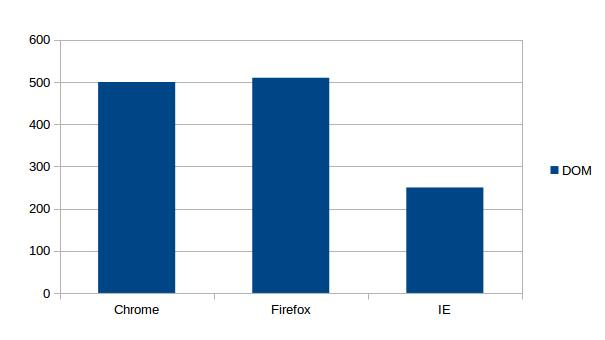
\includegraphics[width=\textwidth]{assets/browser_comp_dom} 
	\caption{Browser-Vergleich DOM}
	\label{browser_comp_dom}
\end{figure}
\newpage
\section{Fazit}
Abschließend lässt sich sagen, dass alle hier vorgestellten Technologien Vor- und Nachteile haben, genauso wie Einsatzgebiete, in denen sie sehr gut verwendet werden können. SVG und DOM können mit sehr wenig Aufwand und einer schlichten API sehr schöne Grafiken und Animationen mit vielen und komplexen Effekten darstellen. Dafür sind diese Techologien nicht geeignet für schnelle Spiele, bei denen sich viele Objekte unvorhersehbar bewegen. Hier bieten sich Canvas oder WebGL an. Canvas hat eine stärkere Verbreitung als WebGL und eine einfache API mit einer flachen Lernkurve, die den Einstieg leicht macht. WebGL bietet dagegen die volle Komplexität von OpenGL, was den Einstieg schwierig macht. Dafür sind die Möglichkeiten nur durch die Hardware selbst begrenzt - bei ordentlicher Optimierung ist die Performance von WebGL unerreicht, wobei sich gefragt werden muss, ob dieser Vorteil schwerer wiegt als die Vorteile von Canvas; für viele Anwendungszwecke reicht die Performance von Canvas aus und man kann die größere Entwicklungsgeschwindigkeit nutzen. Welche Technologie eingesetzt werden soll, hängt stark vom Verwendungszweck ab; Canvas bietet jedoch einen guten Kompromiss aus beiden Welten; eine \emph{High Level API} für einfaches Arbeiten mit komplexen Effekten und trotzdem eine gute Performance, die für viele Anwendungszwecke ausreicht.
\section{Ausblick}
Web-Anwendungen, und damit auch Web-Spiele, sind hier und werden auch so schnell nicht wieder verschwinden. Daher ist es garantiert, dass die behandelten Technologien verbessert und weiterentwickelt werden. Vor allem WebGL wird aufgrund der Möglichkeiten, die sonst nur in nativen Anwendungen möglich sind, in Zukunft eine große Rolle spielen.

Ein noch zu lösendes Problem für die Zukunft ist die weitere Verbesserung der Performance gegenüber nativen Anwendungen; WebGL ist immer noch deutlich langsamer als zum Beispiel C++-Programme. Zusätzlich gibt es immer noch Browser, die WebGL oder sogar Canvas noch nicht unterstützen; wahrscheinlich wird sich dieses Problem in den nächsten Jahren von selbst lösen.
\end{document}
